%\vspace{-4mm}

\section{Empirical Results on Pre-trained DNNs}
\label{sxn:emp}

\nred{TOO LONG for a 10 page paper...move extra results to  Appendix}

(((
\charles{
In this study, we only need to consider Linear and 2D Convolutional (Conv2D) layers because we will only examine series of commonly
available, open source, pre-trained DNNs with these kinds of layers.  We describe these pre-trained models in detail below;
briefly examine the VGG series (VGG11, VGG13, VGG1, VGG19), with and without BatchNorm, the complete set of
available ResNet models ranging from ResNet10 to ResNet152(b), and a wide range of other models.  All models have
been trained on ImageNet, and reported test accuracies are available.  For our analysis, we do not needs to retrain these
models, and we do not even need access to the test data.  }
\michael{This par below.}
)))

(As illustrated in Figure~\ref{fig:vgg_lognorms}, this 
(average log norm of the weight matrices of Eqn.~(\ref{eqn:av_log_norm}))
metric is a relatively good complexity metric for comparing the test accuracies of different, pre-trained DNNs in the same series.)
\michael{Do we use this elsewhere, and probably this comment elsewhere.}


\paragraph{VGG and VGG\_BN Models.}

We start by looking at the VGG class of models, including VGG11, VGG13, VGG16, and VGG19, and their counterparts with Batch Normalization, VGG11\_BN, VGG13\_BN, VGG16\_BN and VGG19\_BN.  
See Figures~\ref{fig:vgg_lognorms} and~\ref{fig:vgg_alphahat} as well as Table~\ref{table:models_VGG} for details.
XXX.  SOME COMMENTS.

\begin{table}[t]
\small
\begin{center}
\begin{tabular}{|p{1in}|c|c|c|c|c|c|c|}
\hline
Architecture 
 & Model &Top1 
 & Top5 & $L$ & $N_{\alpha}$ & $\hat{\alpha}$ \\
\hline
VGG11 & VGG11 & & & & & \\
  & VGG11 BN & & & & & \\
\hline
VGG13 & VGG13 & & & & & \\
  & VGG13 BN & & & & & \\
\hline
VGG16 & VGG16 & & & & & \\
  & VGG16 BN & & & & & \\
\hline
VGG19 & VGG19 & & & & & \\
  & VGG19 BN & & & & & \\
\hline
\end{tabular}
\end{center}
\caption{Results for VGG Series of Architectures and DNN Models.}
\label{table:models_VGG}
\end{table}


\paragraph{ResNet Models.}

Next we look at the ResNet class of models. 
See
Figures~\ref{fig:resnet_lognorms}
and~\ref{fig:resnet_alphahat}
as well as
Table~\ref{table:models_resnet}
for details.
XXX.  SOME COMMENTS.

\begin{figure}[!htb]
   \centering
   \subfigure[log Frobenius norm $\langle\log\Vert\mathbf{W}\Vert_{F}\rangle$]{
      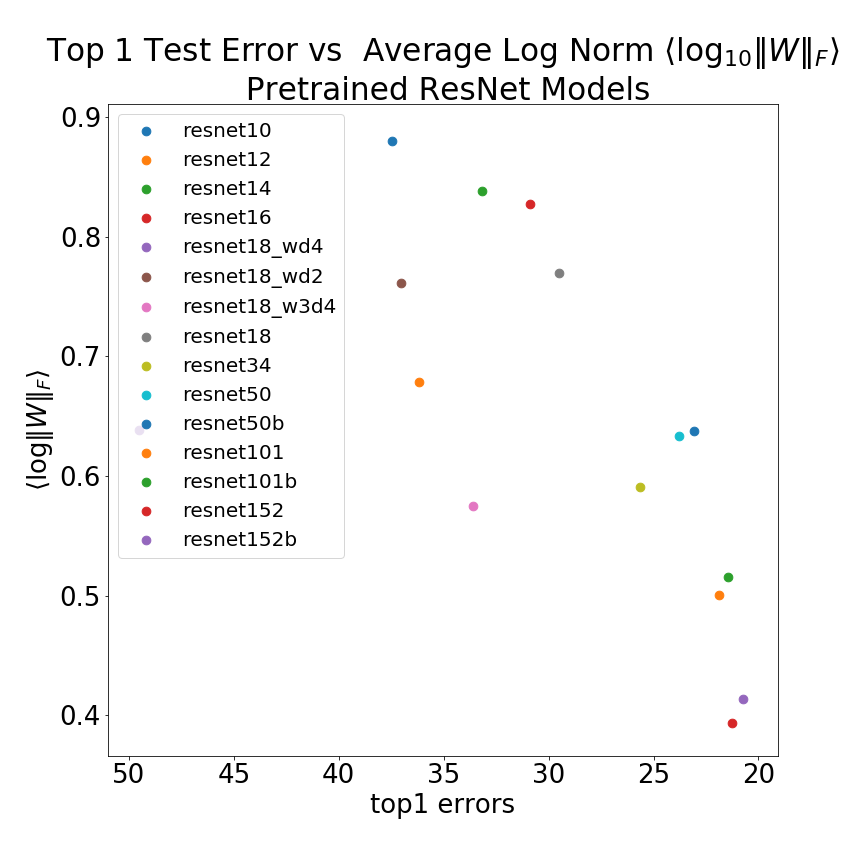
\includegraphics[scale=0.30]{img/ResNet_top1-lognorms.png}
      \label{fig:resnet_lognorms}
   }
   \subfigure[weighted average PL exponent $\hat{\alpha}$]{
      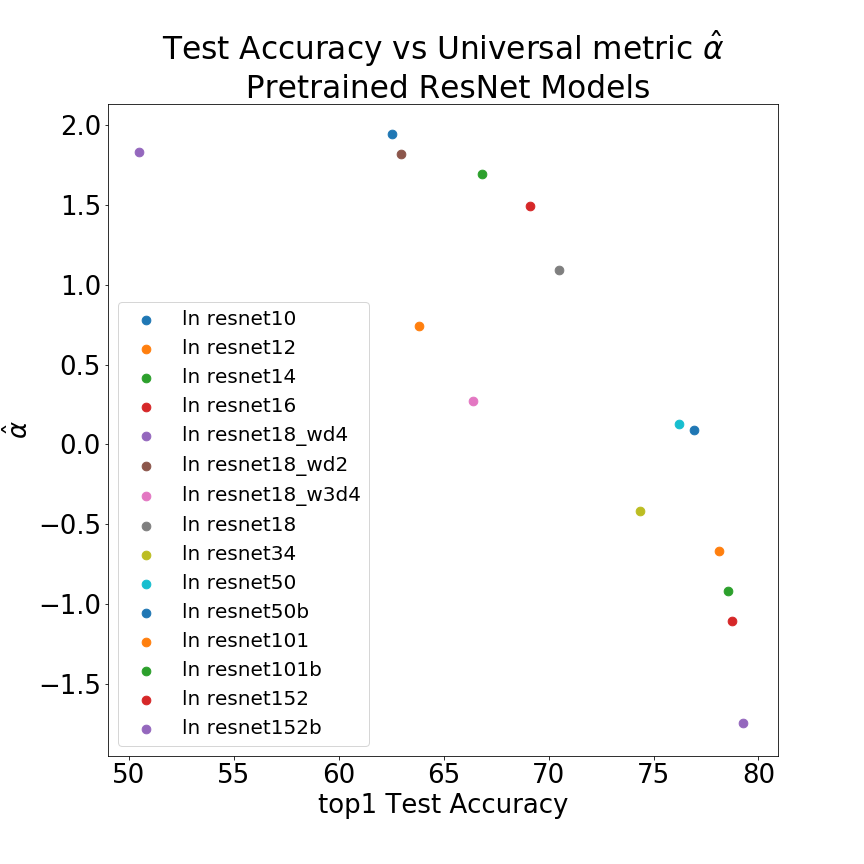
\includegraphics[scale=0.30]{img/ResNet-w_alphas.png}
      \label{fig:resnet_alphahat}
   }
   \caption{
      Pre-trained
      ResNet Series of Architectures and DNNs.  
      Top 1 Test error versus
      average log Frobenius norm $\langle\log\Vert\mathbf{W}\Vert_{F}\rangle$ (in (\ref{fig:resnet_lognorms}))
      or
      weighted average PL exponent $\hat{\alpha}$ (in (\ref{fig:resnet_alphahat})).
           }
   \label{fig:resnet}
\end{figure}

\begin{table}[!htb]
\small
\begin{center}
\begin{tabular}{|p{1in}|c|c|c|c|c|c|c|}
\hline
Architecture 
 & Model
 & Top 1 Error & $\hat{\alpha}$ \\
\hline
ResNet (small)  & resnet10 & 37.46 & \\
& resnet12 & 36.18 & \\
& resnet14 & 33.17 & \\
& resnet16 & 30.9 & \\
\hline
ResNet18 & resnet18\_wd4 & XX & \\
& resnet18\_wd2 & XX & \\
& resnet18 \_wd3d4& XX & \\
& resnet18 & XX & \\

\hline
ResNet34 & resnet34 & 25.66 & \\
\hline
ResNet50 & resnet50 & 23.79 & \\
& resnet50b &  & \\

\hline
ResNet101 & resnet101 & XX.XX & \\
& resnet101b & XX.XX & \\
\hline
ResNet152 & resnet152 & XX,XX & \\
& resnet152b & XX,XX & \\
\hline
\end{tabular}
\end{center}
\caption{Results for ResNet Series of Architectures and DNN Models.
         \michael{Are we going to have the same set of cols for ResNet at least that we had for VGG.}
        }
\label{table:models_resnet}
\end{table}


\paragraph{More Pre-trained Models.}

Here are results for more pre-trained models.
See
Table~\ref{table:models_more}
as well as 
Figure~\ref{fig:models_more} 
for details.
XXX.  SOME COMMENTS.

\begin{table}[!htb]
\small
\begin{center}
\begin{tabular}{|p{1in}|c|c|c|c|c|c|c|}
\hline
Architecture 
 & Model
 & Test Accuracy \\
\hline
GoogLeNet & & \\
\hline
ResNeXt & & \\
\hline
SqueezeNet & & \\
\hline
\end{tabular}
\end{center}
\caption{Results for more models.
         \michael{Why is this split off from the next table.}
        }
\label{table:models_more}
\end{table}

\begin{figure}[!htb]
   \centering
   \subfigure[DenseNet] {
       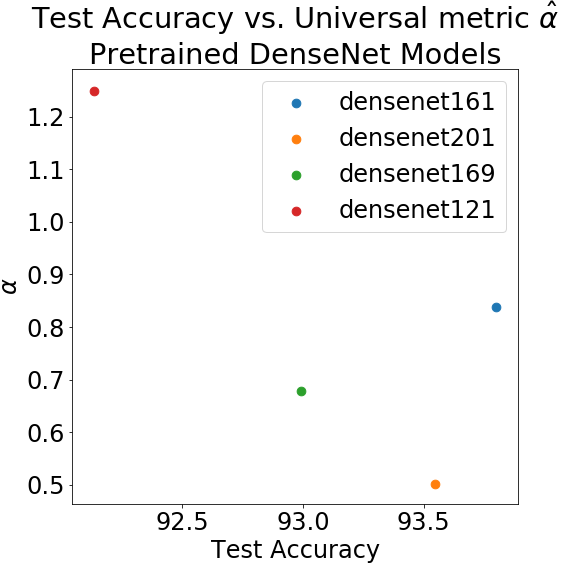
\includegraphics[scale=0.30]{img/densenet-pytorch-w_alphas.png} 
       \label{fig:densenet}
   }
   \subfigure[SqueezeNet]{
       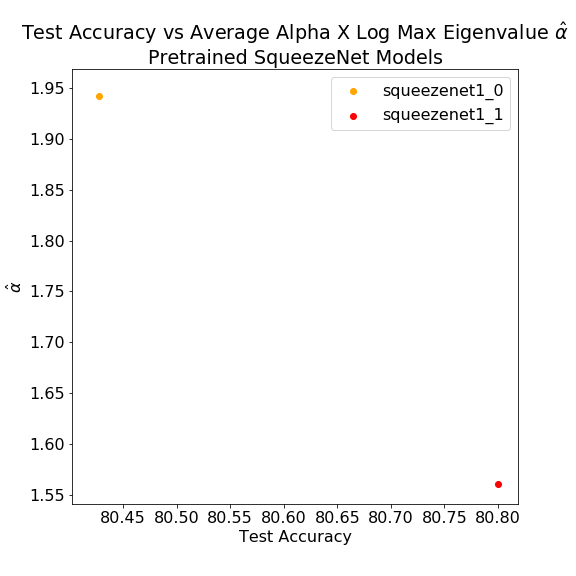
\includegraphics[scale=0.30]{img/squeezenet-pytorch-w_alphas.png} 
       \label{fig:squeezenet}
   }
   \caption{
      Pre-trained 
      Densenet and SqueezeNet PyTorch 
      Models.
      Test Accuracy versus
      $\hat{\alpha}$.
           }
   \label{fig:models_more}
\end{figure}


\paragraph{Still More Pre-trained Models.}

Here are results for still more pre-trained models.
See
Table~\ref{table:models_still_more}
as well as
Figures~\ref{fig:still_more_1} and \ref{fig:still_more_2}
for details.
XXX.  SOME COMMENTS.


\begin{table}[!htb]
\small
\begin{center}
\begin{tabular}{|p{1in}|c|c|c|c|c|c|c|}
\hline
Architecture 
 & Model
 & Top 1 Error \\
 \hline
 DenseNet & densenet121 & 25.57 & \\
& densenet161 & 22.86 & \\
& densenet169 & 24.4 & \\
& densenet201 & 23.1 & \\\hline
DPN & dpn68 & 24.17 & \\
& dpn98 & 20.81 & \\
& dpn131 & 20.54 & \\
\hline
MeNet & menet108\_8x1\_g3 & 43.92 & \\
& menet128\_8x1\_g4 & 43.95 & \\
& menet228\_12x1\_g3 & 33.57 & \\
& menet256\_12x1\_g4 & 33.41 & \\
& menet348\_12x1\_g3 & 30.1 & \\
& menet352\_12x1\_g8 & 33.31 & \\
& menet456\_24x1\_g3 & 28.4 & \\
\hline
MobileNet & mobilenet\_wd4 & 46.26 & \\
& mobilenet\_wd2 & 36.3 & \\
& mobilenet\_w3d4 & 33.54 & \\
& mobilenet\_w1 & 29.86 & \\
\hline
MobileNetV2 & mobilenetv2\_wd4 & 49.72 & \\
& mobilenetv2\_wd2 & 36.54 & \\
& mobilenetv2\_w3d4 & 31.89 & \\
& mobilenetv2\_w1 & 29.31 & \\
\hline
FDMobileNet & fdmobilenet\_wd4 & 55.77 & \\
& fdmobilenet\_wd2 & 43.85 & \\
& fdmobilenet\_w1 & 34.7 & \\
\hline
SE-ResNet & seresnet50 & 22.47 & \\
& seresnet101 & 21.88 & \\
& seresnet152 & 21.48 & \\
\hline
SE-ResNeXt & seresnext50\_32x4d & 21.0 & \\
& seresnext101\_32x4d & 19.96 & \\
\hline
ShuffleNet & shufflenetv2\_wd2 & 41.48 & \\
& shufflenetv2\_w1 & 34.39 & \\
\hline
\end{tabular}
\end{center}
\caption{Results for still more models.
         \michael{Why is this split off from previous table.}
         \michael{Why is CondenseNet missing.}
         \michael{Why Test Accuracy for others and Top 1 Error here.}
        }
\label{table:models_still_more}
\end{table}


\begin{figure}[!htb]
   \centering
   \subfigure[CondenseNet]{
       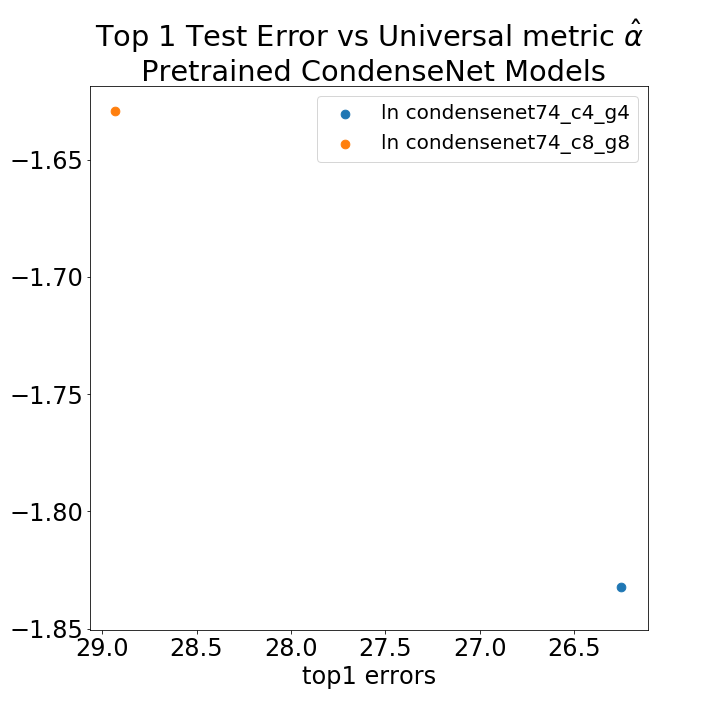
\includegraphics[scale=0.19]{img/CondenseNet-w_alphas.png} 
       \label{fig:densenet-small}
   }
   \subfigure[DPN]{
       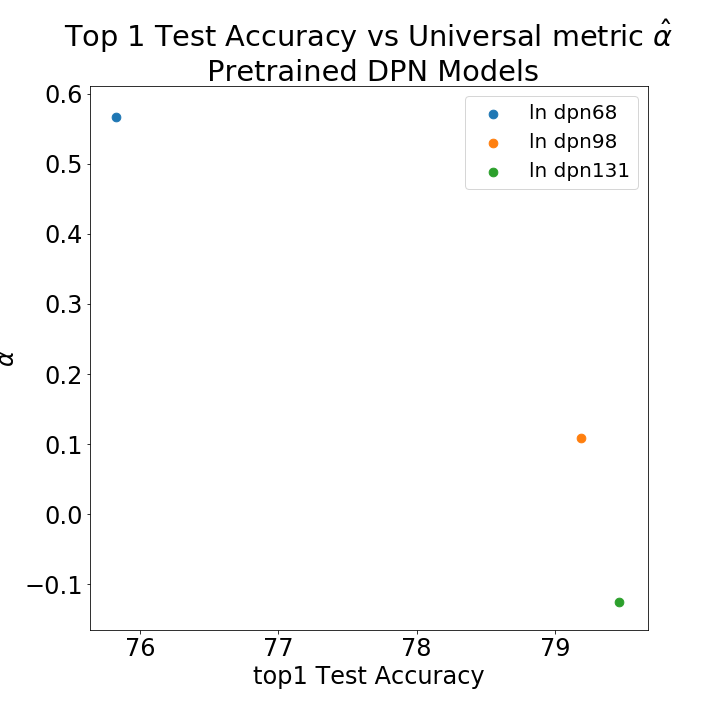
\includegraphics[scale=0.19]{img/DPN-w_alphas.png} 
       \label{fig:dpn-net}
   }
   \subfigure[ShuffleNet]{
      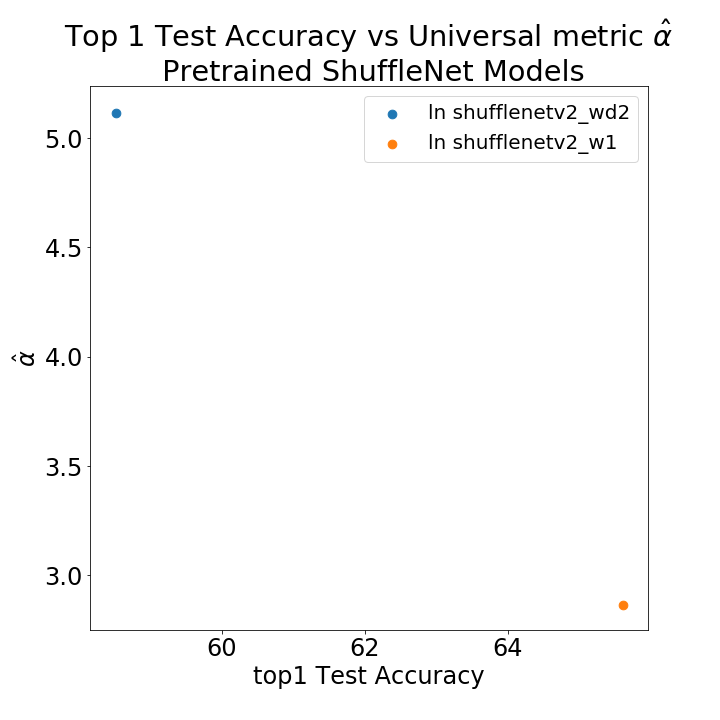
\includegraphics[scale=0.19]{img/ShuffleNet-w_alphas.png}
      \label{fig:shufflenet-small}
   }
   \caption{
      Pre-trained 
      CondenseNet, DPN, and ShuffleNet
      Models.
      Top 1 Test error versus
      $\hat{\alpha}$.
           }
   \label{fig:still_more_1}
\end{figure}


\begin{figure}[!htb]
   \centering
   \subfigure[MobileNet]{
      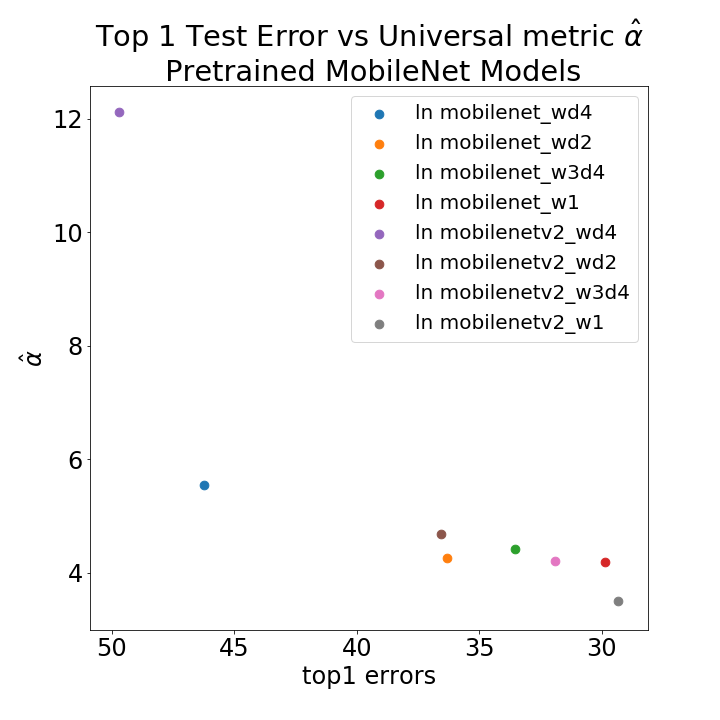
\includegraphics[scale=0.19]{img/MobileNet-w_alphas.png} 
      \label{fig:resnet-small}
   }
   \subfigure[SeResNet]{
      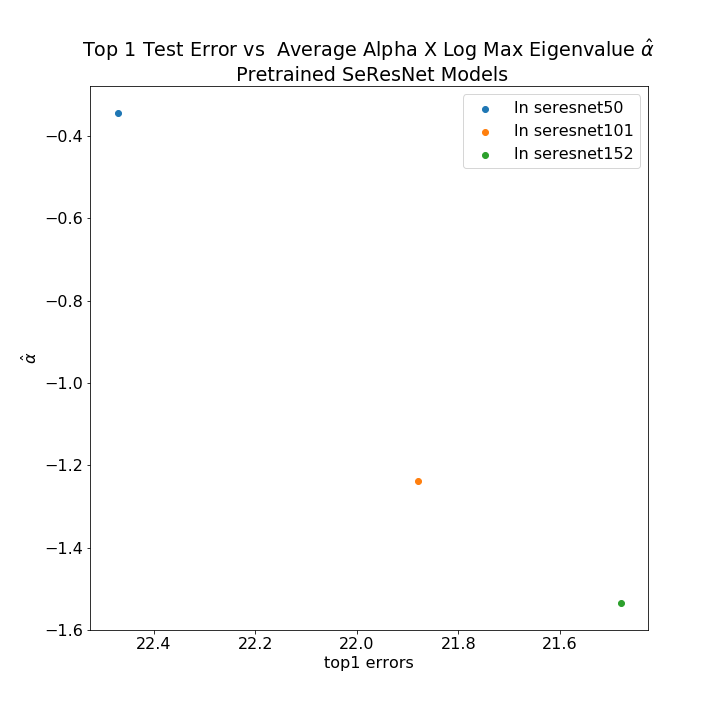
\includegraphics[scale=0.19]{img/SeResNet-w_alphas.png}
      \label{fig:shufflenet-small}
   }
   \subfigure[SeResNeXt]{
      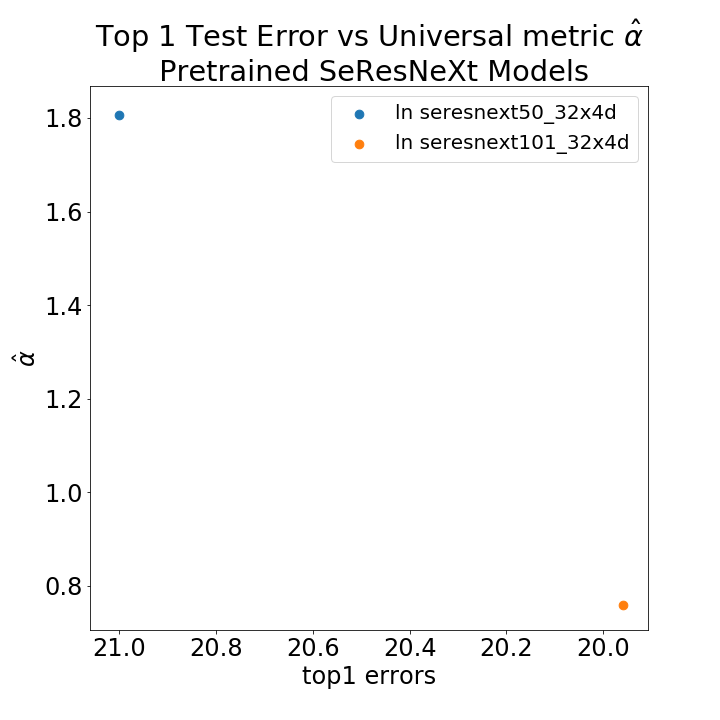
\includegraphics[scale=0.19]{img/SeResNeXt-w_alphas.png}
      \label{fig:shufflenet-small}
   }
   \caption{
      Pre-trained 
      MeNet, SeResNet, and SeResNeXt
      Models.
      Top 1 Test error versus
      $\hat{\alpha}$.
           }
   \label{fig:still_more_2}
\end{figure}


\paragraph{Counterexamples.}
There are of course exceptions here and there.
See
Figure~\ref{fig:counter-examples}
as well as 
Table~\ref{table:models_still_more}
for details on the counterexamples.
XXX.  COMMENTS.

\begin{figure}[!htb]
   \centering
   \subfigure[ResNeXt]{
      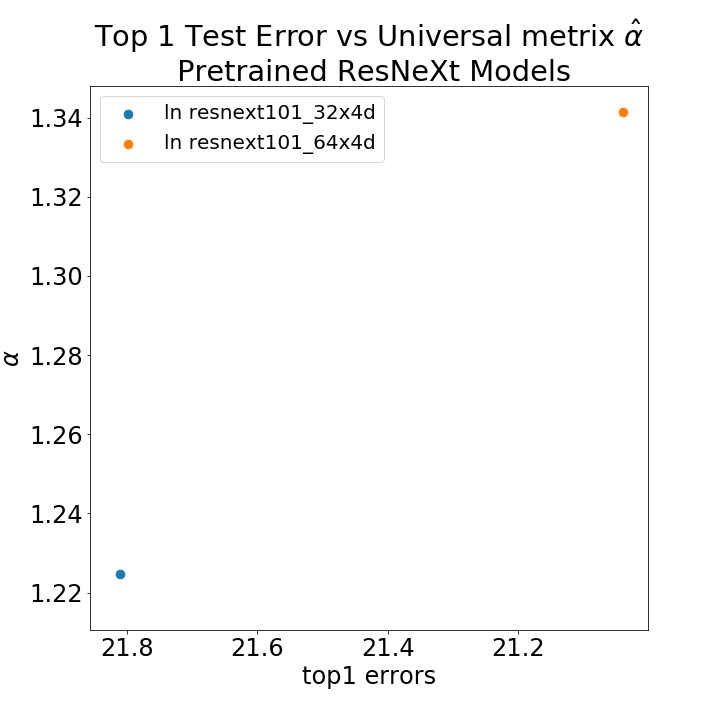
\includegraphics[scale=0.19]{img/ResNeXt-w_alphas.png} 
      \label{fig:resnet-small}
   }
   \subfigure[MeNet]{
      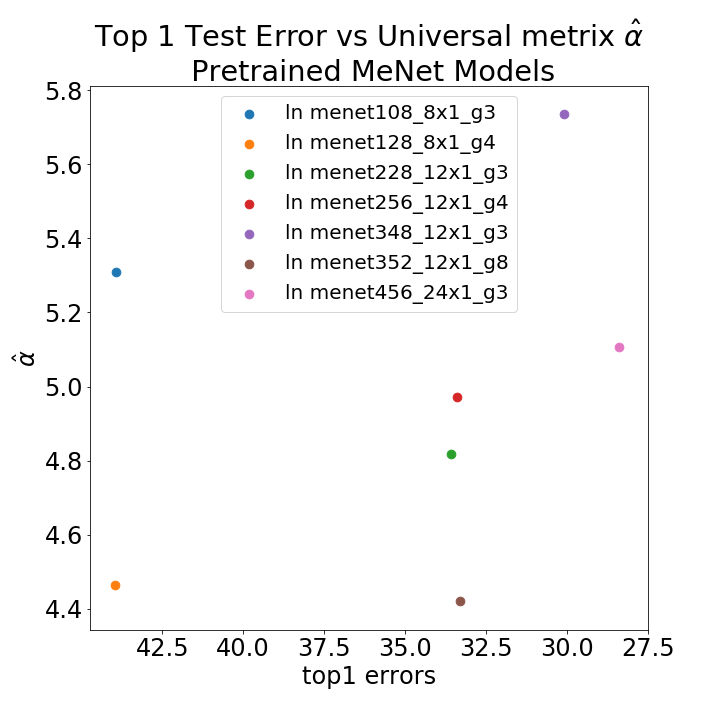
\includegraphics[scale=0.19]{img/MeNet-w_alphas.png} 
      \label{fig:menet-net}
   }
   \subfigure[FDMobileNet]{
      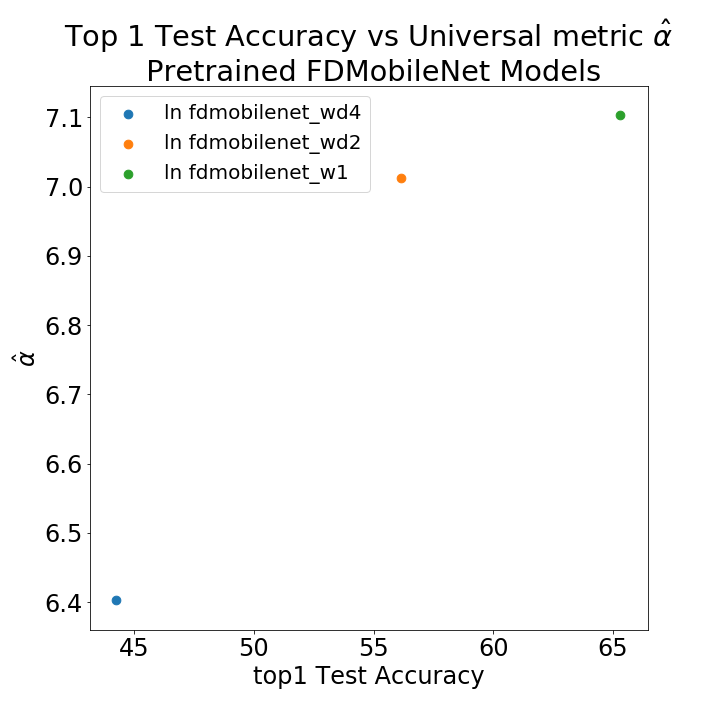
\includegraphics[scale=0.19]{img/FDMobileNet-w_alphas.png} 
      \label{fig:resnet-small}
   }
   \caption{
      Pre-trained 
      ResNeXt, MeNet, and FDMobileNet
      Models 
      that provide counterexamples to our main trends.
      Top 1 Test error versus
      $\hat{\alpha}$.
           }
   \label{fig:counter-examples}
\end{figure}


